\section{Klassen}
%    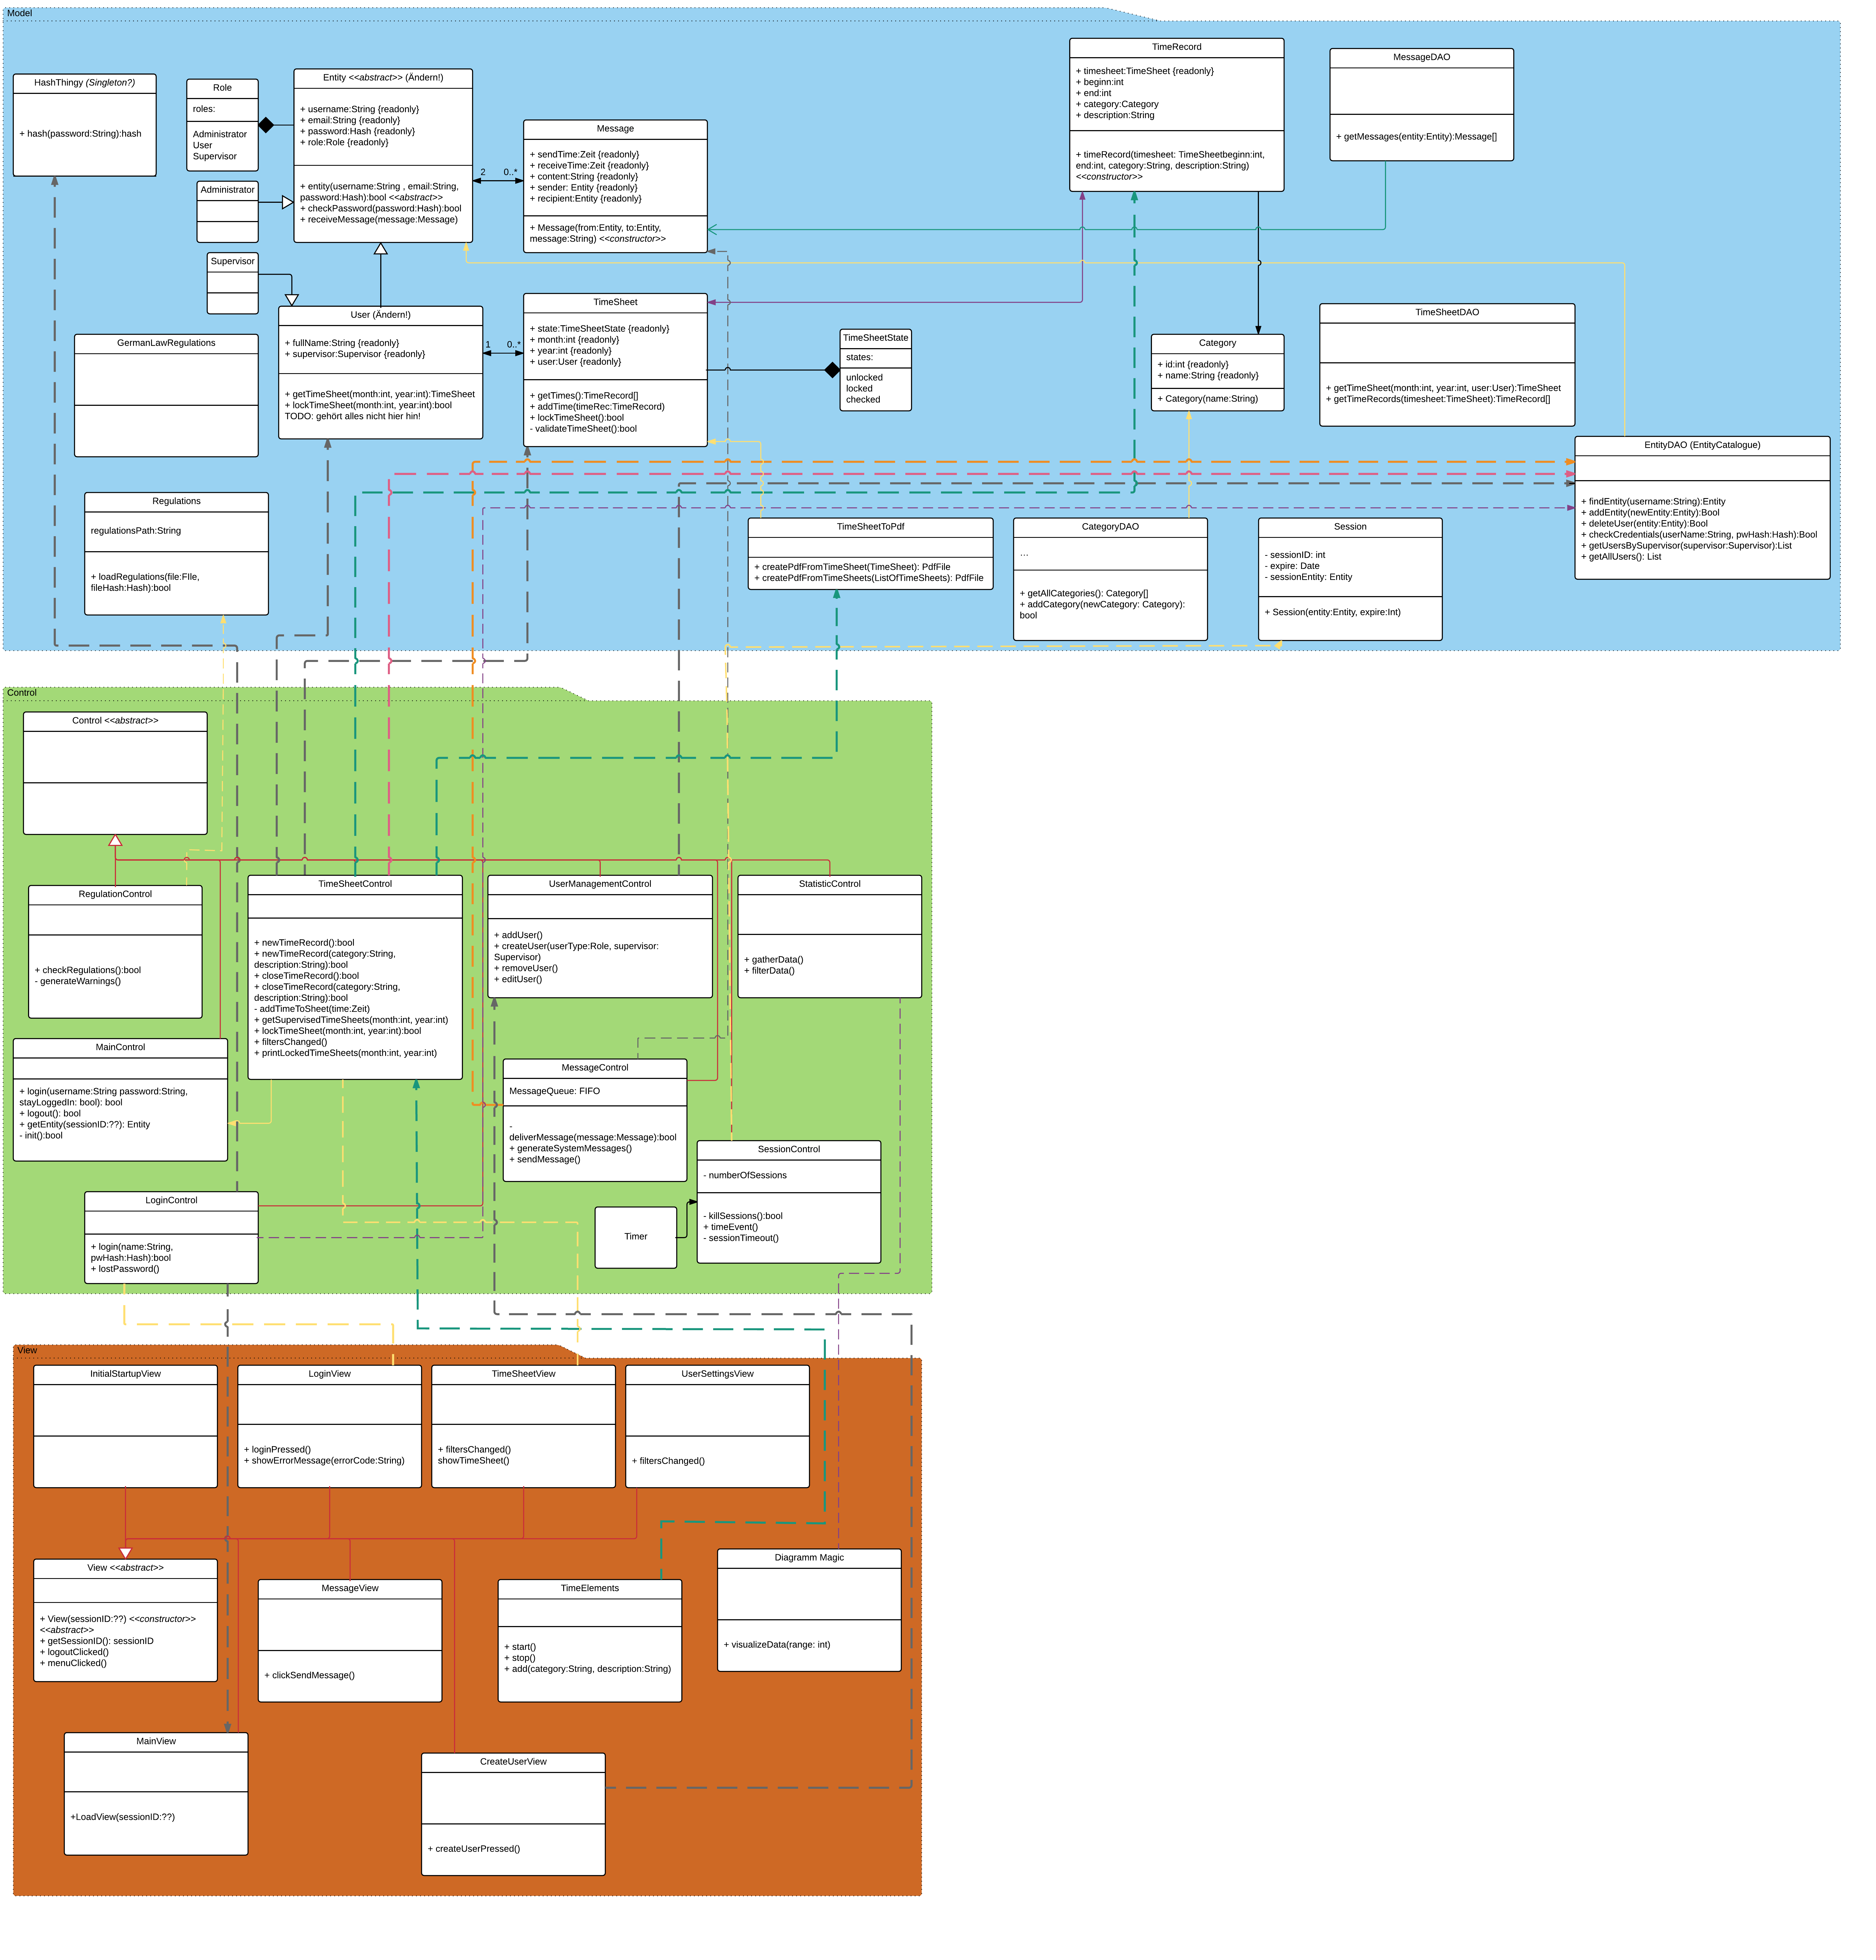
\includegraphics[width=\linewidth]{Diagramms/class/overview.png}\\
    TODO Bild des kompletten Klassendiagrams
    \newpage
    \subsection{Model}
        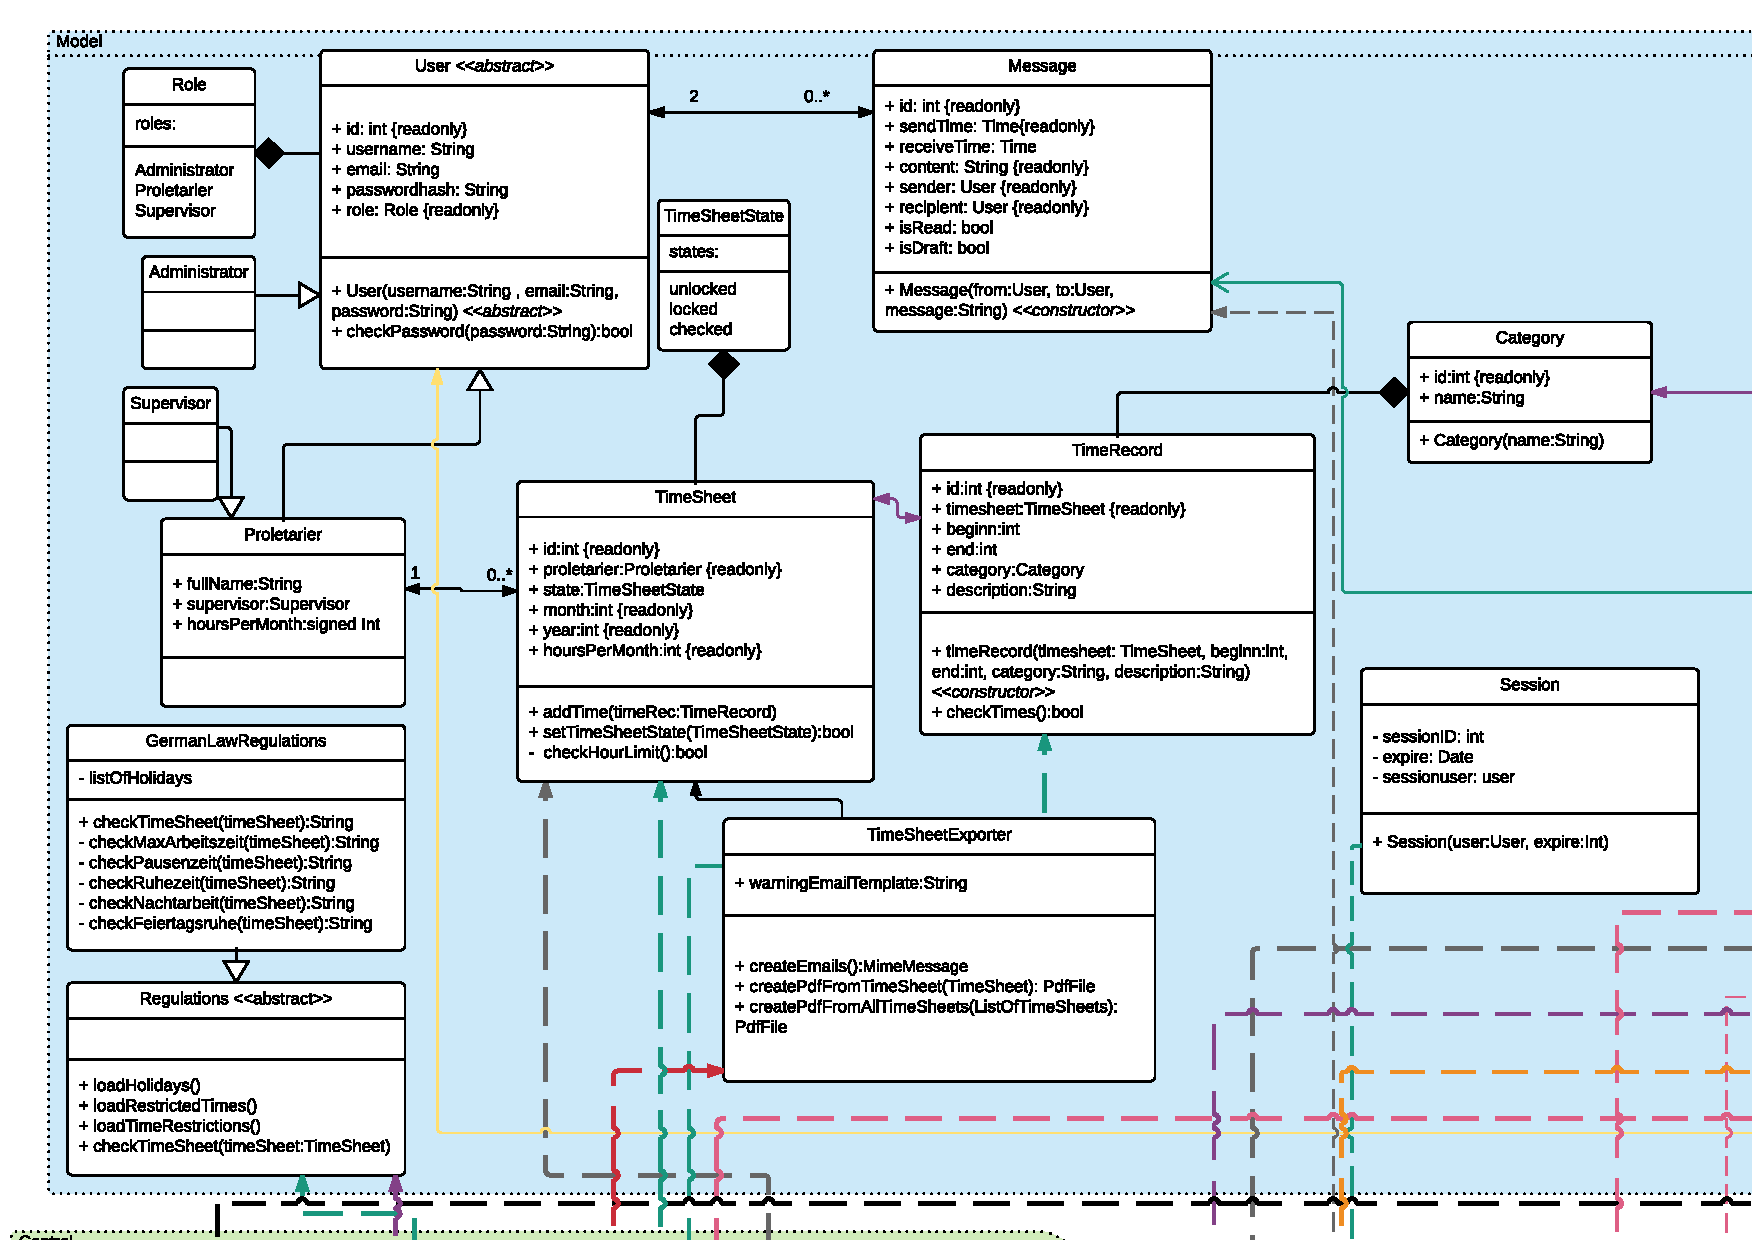
\includegraphics[width=\linewidth,page=1]{Diagramms/class/model.pdf}\\
        \includegraphics[width=\linewidth,page=2]{Diagramms/class/model.pdf}\\
        \begin{itemize}
            \item{Company}
                Speichert Informationen über die Firma in der die Zeiterfassung betrieben wird.
                \begin{itemize}
                    \item{}
                \end{itemize}

            \item{Entity}
                Grundform eines Benutzers, stellt grundlegende Daten und Funktionen für Spezialisierte Benutzer bereit.
                Folgende Spezialisierungen sind möglich:
                \begin{itemize}
                    \item{Admin}
                        Stellt Daten für und über den Admin bereit.
                    \begin{itemize}
                        \item{}
                    \end{itemize}

                    \item{User}
                        Stellt Daten für und über den User bereit, darüber hinaus hat der User eine verbing zu dem mit ihm assozierten Zeiterfassungen und Stundenzetteln.
                        \begin{itemize}
                            \item{}
                        \end{itemize}

                    \item{Supervisor}
                        Erweiterung des User um Gruppen von Usern zu verwalten.
                        \begin{itemize}
                            \item{}
                        \end{itemize}

                \end{itemize}
                \begin{itemize}
                    \item{entity\(username:String , email:String, password:Hash\)}
                    \item{checkPassword\(password:Hash\):bool}
                    \item{receiveMessage\(message:Message\)}
                \end{itemize}

            \item{EntityDAO}
                Listet alle vorhanden Entities auf. Enthält Methoden um Entities hinzuzufügen, zu löschen oder zu verändern. Stellt darüber hinaus sicher, dass die alle einträge einzigartig sind.
                \begin{itemize}
                   \item{findEntity\(username:String\):Entity}
                   \item{addEntity\(newEntity:Entity\):Bool}
                   \item{deleteUser\(entity:Entity\):Bool}
                   \item{checkCredentials\(userName:String, pwHash:Hash\):Bool}
                   \item{getUsersBySupervisor\(supervisor:Supervisor\):List}
                   \item{getAllUsers\(\): List}
                \end{itemize}

            \item{Regulations}
                Lädt die gesetzlichen Regularien aus einer Datei und stellt diese für andere Klassen bereit.
                \begin{itemize}
                    \item{checkTimeSheet\(TimeSheet\):String}
                \end{itemize}

            \item{TimeSheet}
                Speichert Zeiterfassungen. Methoden zur Validierung und sicherstellung der unveränderlichkeit sind vorhanden.
                \begin{itemize}
                    \item{getTimes\(\):TimeRecord\[\]}
                    \item{addTime\(timeRec:TimeRecord\)}
                    \item{lockTimeSheet\(\):bool}
                    \item{validateTimeSheet\(\):bool}
                \end{itemize}

            \item{TimeSheetState}
                Zustände, die beschreiben, ob ein Stundenzettel verändert werden darf, bzw bereits überprüft wurde.

            \item{TimeRecord}
                Datenhaltung, der Zeiterfassung.
                \begin{itemize}
                   \item{timeRecord(timesheet: TimeSheetbeginn:int, end:int, category:String, description:String)}
                \end{itemize}

            \item{Session}
                Daten die mit einer Login Session assoziert sind(User, ablaufdatum, ...) werden in dieser Klasse gespeichert.
                \begin{itemize}
                    \item{Session(entity:Entity, expire:Int)}
                \end{itemize}

            \item{Category}
                Kategorie, die für die Zeiterfassung benötigt wird
                \begin{itemize}
                    \item{Category(name:String)}
                \end{itemize}

            \item{Categories}
                Liste aller verfügbaren Kategorien.
                \begin{itemize}
                   \item{getAllCategories(): Category[]}
                   \item{addCategory(newCategory: Category): bool}
                \end{itemize}

            \item{Message}
                Nachrichten und damit Verbundene Metadaten können mit dieser Klasse erfasst werden.
                \begin{itemize}
                    \item{Message(from:Entity, to:Entity, message:String)}
                \end{itemize}

            \item{HashThingy}
                Stellt Passwort Hash funktionen bereit.
                \begin{itemize}
                    \item{hash(password:String):hash}
                \end{itemize}

            \item{TimeSheetToPdf}
                Klasse, um Stundenzettel als .pdf zu exportieren.
                \begin{itemize}
                    \item{createPdfFromTimeSheet(TimeSheet): PdfFile}
                    \item{createPdfFromAllTimeSheets(ListOfTimeSheets): PdfFile}
                \end{itemize}

        \end{itemize}

    \subsection{Control}
        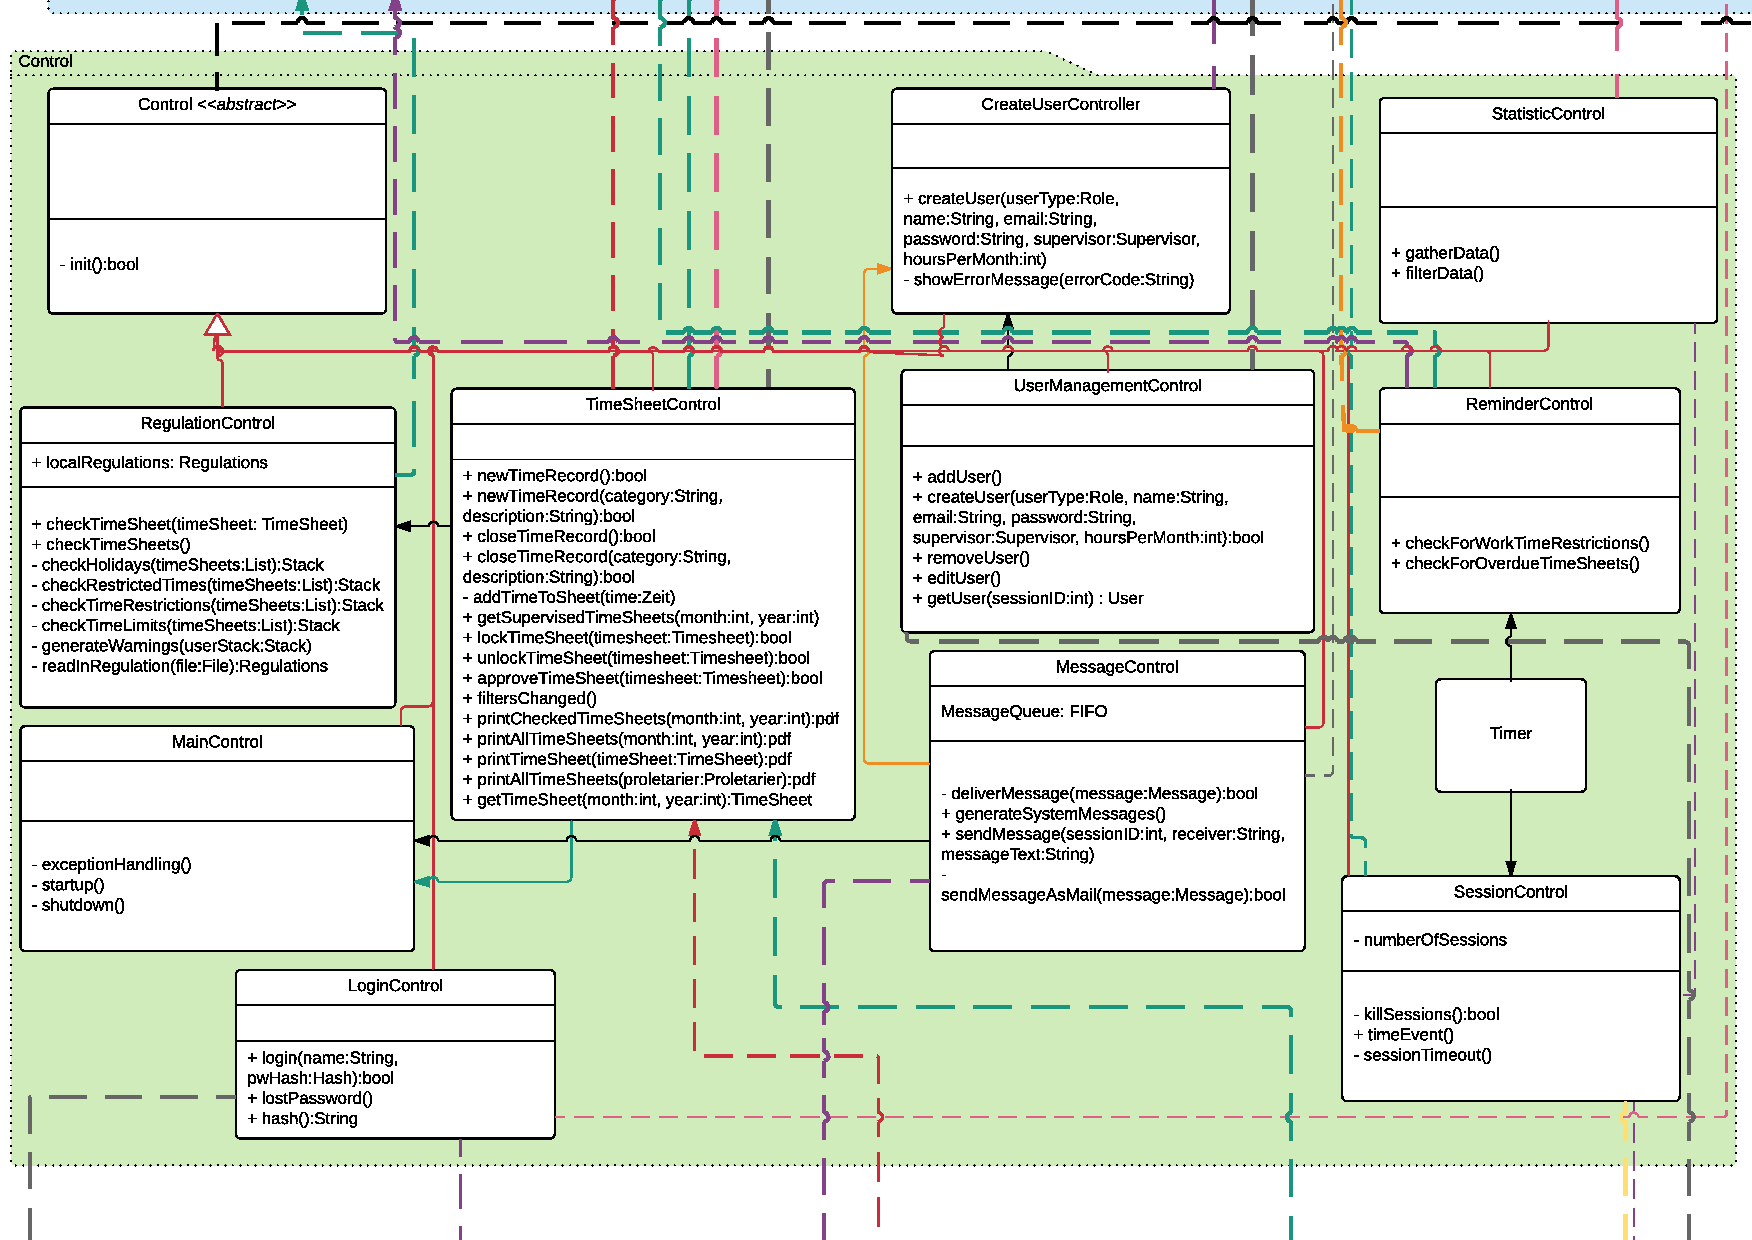
\includegraphics[width=\linewidth]{Diagramms/class/control.pdf}\\
        \begin{itemize}
            \item{Control}
                \begin{itemize}
                    \item{RegulationControl}
                       Überprüft Daten auf Gesetzeskonformität, leitet ebenfalls notwendige Schritte ein.
                       \begin{itemize}
                           \item{checkRegulations():bool}
                           \item{generateWarnings()}
                       \end{itemize}

                    \item{MainControl}
                        Kontroliert den Hauptablauf des Programms.
                        \begin{itemize}
                             \item{login(username:String password:String,  stayLoggedIn: bool): bool}
                             \item{logout(): bool}
                             \item{getEntity(sessionID:??): Entity}
                             \item{init():bool}
                        \end{itemize}

                    \item{TimeSheetControl}
                        Regelt die Erstellung von Stundendaten für den Stundenzettel, darüber hinaus wird auch die abrarbeitung eines fertigen Stundenzettels geregelt.
                        \begin{itemize}
                             \item{newTimeRecord():bool}
                             \item{newTimeRecord(category:String, description:String):bool}
                             \item{closeTimeRecord():bool}
                             \item{closeTimeRecord(category:String, description:String):bool}
                             \item{addTimeToSheet(time:Zeit)}
                             \item{getSupervisedTimeSheets(month:int, year:int)}
                             \item{lockTimeSheet(month:int, year:int):bool}
                             \item{filtersChanged()}
                             \item{printLockedTimeSheets(month:int, year:int)}
                             \item{getTimeSheet(month:int, year:int):TimeSheet}
                        \end{itemize}

                    \item{UserManagementControl}
                        Managed das hinzufügen, löschen und verändern von Benutzern
                        \begin{itemize}
                             \item{addUser()}
                             \item{createUser(userType:Role, supervisor: Supervisor)}
                             \item{removeUser()}
                             \item{editUser()}
                        \end{itemize}

                    \item{LoginControl}
                        Überwacht das korrekte Einloggen von Benutzern.
                        \begin{itemize}
                             \item{login(name:String, pwHash:Hash):bool}
                             \item{lostPassword()}
                        \end{itemize}

                    \item{MessageControl}
                        Stellt Nachrichten zwischen Benutzern (und dem System) zu.
                        \begin{itemize}
                             \item{deliverMessage(message:Message):bool}
                             \item{generateSystemMessages()}
                             \item{sendMessage()}
                        \end{itemize}

                    \item{StatisticControl}
                        Sammelt und generiert Statistiken über die erfassten Stundendaten.
                        \begin{itemize}
                             \item{gatherData()}
                             \item{filterData()}
                        \end{itemize}

                    \item{SessionControl}
                        Kontrolliert offene Sessions und terminiert diese nach ablauf eines gesetzen Zeitraums.
                        \begin{itemize}
                            \item{killSessions():bool}
                            \item{timeEvent()}
                            \item{sessionTimeout()}
                        \end{itemize}
                \end{itemize}
                \begin{itemize}
                     \item{}
                \end{itemize}

            \item{Timer}
            \begin{itemize}
                 \item{}
            \end{itemize}

        \end{itemize}

    \subsection{View}
    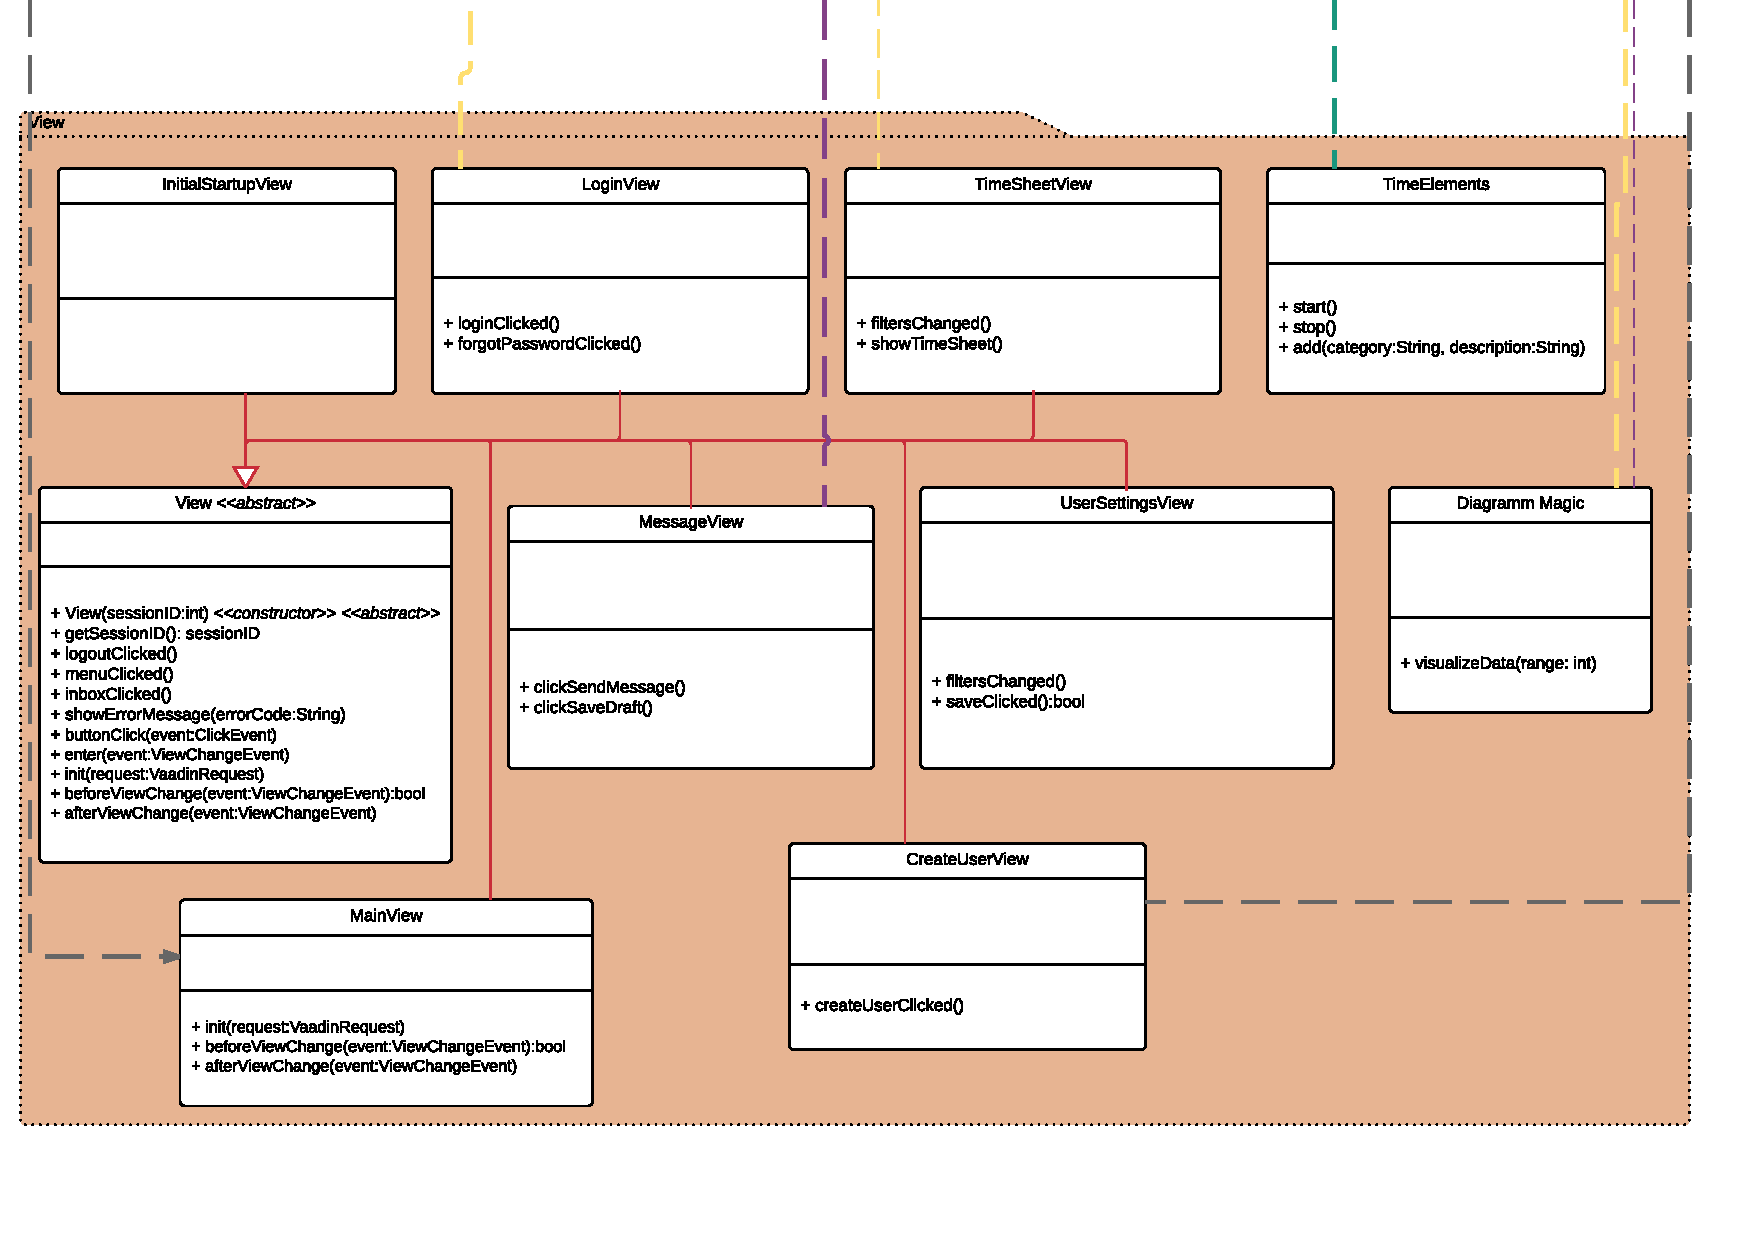
\includegraphics[width=\linewidth]{Diagramms/class/view.pdf}\\
        \begin{itemize}
            \item{View}
                \begin{itemize}
                    \item{LoginView}
                    \begin{itemize}
                        \item{loginPressed()}
                        \item{showErrorMessage(errorCode:String)}
                    \end{itemize}

                    \item{TimeSheetView}
                    \begin{itemize}
                        \item{filtersChanged()}
                        \item{showTimeSheet()}
                    \end{itemize}

                    \item{UserSettingsView}
                    \begin{itemize}
                        \item{filtersChanged()}
                    \end{itemize}

                    \item{MainView}
                    \begin{itemize}
                        \item{LoadView(sessionID:??)}
                    \end{itemize}

                \end{itemize}
                \begin{itemize}
                    \item{View(sessionID:??)}
                    \item{getSessionID(): sessionID}
                    \item{logoutClicked()}
                    \item{menuClicked()}
                \end{itemize}

            \item{Diagramm Magic}
            \begin{itemize}
                \item{visualizeData(range: int)}
            \end{itemize}

            \item{TimeElements}
            \begin{itemize}
                \item{start()}
                \item{stop()}
                \item{add(category:String, description:String)}
            \end{itemize}

        \end{itemize}